\documentclass[10pt,a4paper]{article}
\usepackage[utf8]{inputenc}


\usepackage[francais]{babel}
\usepackage[T1]{fontenc}
\usepackage{amsmath}
\usepackage{amsfonts}
\usepackage{amssymb}
\usepackage{graphicx}
\usepackage{lmodern}
\usepackage{multicol}
\usepackage{tikz}

\author{Pierre \bsc{Donat-Bouillud} Thibaud \bsc{Ehret}}
\title{Lancer de rayons}

% Parler surtout de l'architecture : 
% « Je n'attends pas de vous des démonstrations mathématiques et algorithmiques, mais une réflexion sur 
% les structures de données utilisée, le découpage en classes, les difficultés d'implémentations et les résultats. »

%% ATTENTION : 5 pages max de texte (toutes les images -> en annexe )

\begin{document}

\maketitle

\section*{Introduction} %Situer le problème du lancer de rayon
Le lancer de rayon est 
\section{Organisation du projet} % Parler ici de la hiérarchie de classes et des structures de données, de git, de github, et de Doxygen

% Parler ici de la hiérarchie de classes et des structures de données, de git, de github, et de Doxygen, licence GPL
\subsection{Organisation du travail}
  Nous avons utilisé \emph{git}, couplé à un dépôt \emph{git} sur \emph{github}, qui affiche de jolis graphes de la progression du projet, 
  et a un système d'\emph{issues}, ce qui permet d'assigner des objectifs avec une date. 
   La création de branches a permis de mener efficacement un travail parallèle, et l'outil de résolution des conflits \emph{meld} a grandement contribué à ce que les moments
  de fusion de branches soient extrêmement rapides.
  Le dépôt étant public, il a fallu mettre une licence adaptée : la licence \emph{GPL}.
  
  Le code est commenté avec des commentaires \emph{Doxygen}, ce qui permet de générer automatiquement une documentation au format html.
  
\subsection{Organisation du projet}

\paragraph{Hiérarchie de classe : } 
Les différentes abstractions qui permettent de rendre une scène ont été conçues pour être les plus génériques possibles. Dans la mesure du possible, les différents  objets insérables dans une scène sont une classe abstraite pure : \verb|Solid|, \verb|Light|...
\begin{figure}[h]
\begin{center}
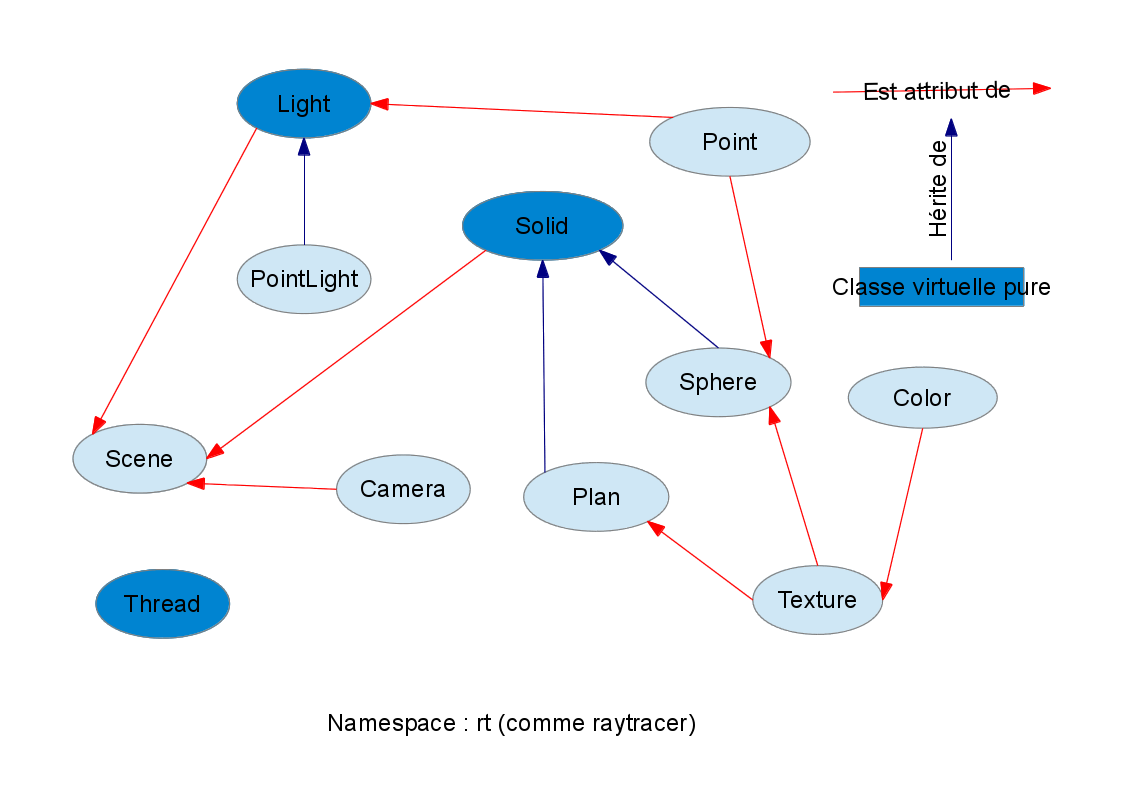
\includegraphics[scale=0.35]{hierarchie.png}
\end{center}
\caption{Hiérarchie de classes.}
\end{figure}

Ainsi, pour créer un nouveau type d'objet, par exemple, une sphère, il faut hériter de \verb|Solid| puis implémenter les quatre méthodes virtuelles 
pures de \verb|Solid| suivantes :

\begin{lstlisting}
virtual bool intersect(const Point& pos, const vector& vect) const = 0;

virtual Point getIntersection(const Point& point, const vector& vect) const = 0;

virtual Point autreCote(const Point& point, const vector& vect,	const Point& act) const = 0;

virtual vector getNormal(const Point& p, const vector& v) const = 0;
\end{lstlisting}

Pour créer un nouveau type de lampe, comme une lumière ponctuelle, il faudra hériter de \verb|Light|, et implémenter :
\begin{lstlisting}
virtual color illuminate(const Point& point, const Solid* m, const vector vision) const = 0;
\end{lstlisting}

Toutes les classes du lanceur de rayons sont placées dans l'espace de nom \emph{rt}. Pour créer une scène particulière, il est
conseillé de dériver une classe \emph{MyScene}  de \emph{Scene}, ce qui permet de gérer les allocations et désallocations 
mémoire des objets dans la scène proprement. Ces classes, qui sont du ressort de l'utilisateur, ne se trouvent donc pas dans l'espace
 de nom \emph{rt}.

\paragraph{Structures de données : }
Les structures de données utilisées pour conserver les objets dans une scène (lampes, solides), sont des \verb|vector|\footnote{sic} : 
\begin{lstlisting}
std::vector<Solid*> objets;
std::vector<Light*> lights;
\end{lstlisting}
Les \verb|vector|\footnote{sic} ont l'inconvénient d'occasionner un temps de recherche linéaire (voir table \ref{tempsSphères}) de l'intersection entre les objets dans la scène et un rayon lancé. 
Des structures de données plus efficaces mais plus complexes, \emph{octree} et \emph{voxels}, existent.

\begin{table}
\begin{center}
\begin{tabular}{|c|c|c|c|c|c|}
\hline 
Nombre de sphères & 10 & 50 & 100 & 500 & 1000 \\ 
\hline 
Temps de rendu (s) & 6 & 23 & 41 & 190 & 387 \\ 
\hline 
\end{tabular} 
\end{center}
\caption{Évolution du temps de rendu en fonction du nombre de sphères dans la scène.} \label{tempsSphères}
\end{table}

\section{Illumination} % Parler des difficultés d'implémentations et des résultats visuels, changer de titre ?
% Court !! Rapidement le principe, rapidement l'implémenation. Rapidement expliquer Phong (une jolie formule ?)
\subsection{Les buts et les difficultés}
Nous avons cherché à utiliser une méthode permettant d'avoir un rendu réaliste, tout en n'étant pas trop compliqué à implémenter, et qui permette de faire certaines améliorations comme rajouter la transparence ou la réflection des rayons sur les sphères. C'est pour cela que nous avons choisi d'implémenter l'illumination de Phong.

\subsection{L'illumination de Phong}

L'illumination de Phong se découpe en plusieurs composantes : l'illumination ambiante, l'illumination spéculaire et l'illumination diffuse.
\begin{enumerate}
\item La lumière ambiante est constante dans l'espace et représente les parasites lumineux provenant de tous les points de l'espace. Nous l'avons considérée comme nulle dans notre projet ; elle est en général, pour plus de réalisme, gérée par des techniques telle que photon-mapping que nous n'avons pas eu le temps d'implémenter.
\item La lumière spéculaire est la lumière qui s'est réfléchie sur l'objet avant de parvenir à la caméra. Une réflexion plus ou moins parfaite peut être obtenue grâce à un facteur de brillance $\alpha$. En considérant les vecteurs unitaires comme définis sur le schéma \ref{speculaire}, l'intensité de la lumière parvenant à la caméra est alors $<\vec{R}|\vec{V}>^{\alpha} i_{s} k_{s}$ où $i_{s}$ l'intensité de la lumière incidente est $k_{s}$ une constante liée au matériau. En pratique, nous avons appliqué cette formule pour chaque canal RGB et choisi les intensités comme les valeurs des canaux RGB de la lumière incidente et $k_{s}$ proportionnel au canal de la couleur naturel de l'objet.
\item La lumière diffuse correspond à la partie de la lumière qui est absorbée par l'objet avant d'être réémise de façon isotrope et uniformément dans l'espace. En considérant les mêmes notations que sur le schéma \ref{diffuse}, l'intensité réémise est alors $i_{d}k_{d}<\vec{L}|\vec{N}>$ \footnote{Avec les mêmes remarques que pour la lumière spéculaire.}
\end{enumerate}

Les sources de lumière multiples sont gérées de la manière suivante : pour chaque source, l'intensité reçue est calculée puis tout est sommé \footnote{Pour rester dans les canaux RGB, l'intensité reçue possible est majorée dans notre implémentation.}.

La formule finale pour l'intensité est alors \[i = \sum_{l \in lumieres}(<\vec{R}|\vec{V}>^{\alpha} {i_{s}}_{l} k_{s} + {i_{d}}_{l}k_{d}<\vec{L}|\vec{N}>)\].

Les résultats après implémentation sont les captures des figures \ref{phong} suivantes.

\section{Améliorations} % Parler ici du multithreading, des réflexions et transparence, et de l'anticrénelage

\subsection{La réflection}
Nous avons implémenté la réflection de la lumière sur de multiples sphères avant d'accéder à la source de lumière pour pouvoir ajouter un effet miroir aux sphères. Pour cela, nous avons considéré que le rayon se réfléchissait parfaitement sur la sphère avant de continuer. Cela permet de calculer l'éclairement par récurrence : la lumière arrivant en un point est celle que l'on recevrait avec une caméra placée en ce point et avec une direction celle du vecteur réfléchi \ref{reflection}.

L'implémentation a donné des résultats comme celui-ci \ref{ereflection}.

\subsection{La transparence}
  La transparence des objets a été aussi implémentée : la possibilité de voir un objet à travers un autre. Pour cela, un rayon peut traverser un objet, ce qui entraîne une diminution d'intensité. Les lois de Snell-Descartes ont ensuite été ajoutées, pour avoir la réfraction dans les sphères et gérer des effets comme celui de la lumière qui traverse une boule en verre \ref{refraction}.
Les résultats sont assez réalistes :  \ref{erefraction}.

\subsection{Anti-crénelage}
  Les images rendues par le lanceur de rayons présentent le long de leurs contours des bords crénelés.
Il est possible de réduire ce crénelage disgracieux en utilisant le suréchantillonage, en l'occurence, $\times 8$ : on calcule en plus 
 du pixel considéré huit autres pixels, répartis équitablement autour de ce pixel, et puis on effectue la moyenne des couleurs.
Cette méthode demande beaucoup de calculs par rapport à d'autres méthodes, mais est très simple à mettre en place.
  Les résultats son convaincants : voir la figure \ref{crenelage}.
 
\subsection{Multithreading}
  Les temps de rendus devenant prohibitifs, il a paru intéressant d'utiliser à leur plein potentiel les machines multicoeurs, et multiprocesseurs.
  Le lancer de rayon est d'ailleurs extrêmement facilement parallélisable : chaque calcul de la couleur d'un pixel est indépendant de celui des 
  autres.
  
  Notre rendu multithreadé utilise une bibliothèque C, \emph{pthread} \footnote{Posix Threads}, qu'il a fallu, pour que le code soit plus idiomatique de C++, 
  encapsuler dans une classe : \emph{Thread}. Pour utiliser la fonction \verb|pthread_create| qui prend en argument un pointeur de fonction, passer une méthode de classe
  n'était pas possible, car celles-ci prennent en argument un pointeur caché vers l'objet dont elles sont méthodes. Il a donc fallu créer une méthode statique privée.
  
  Pour lancer un thread, il faut hériter de la classe \emph{Thread}, et implémenter la méthode :
  \begin{lstlisting}
  virtual void run() = 0;
  \end{lstlisting}
  
  Une fonction détecte le nombre de coeurs disponibles, qui est supposé être une puissance de deux.
  
  Le découpage de l'image s'effectue alors en prenant, avec $ n = \log_2(nbThreads) $ et $ m = nbThreads / n$, en une grille de $n \times m$ rectangles.
  
 Une augmentation de la vitesse de rendu est finalement bien obtenue (voir table \ref{tempsRendu}).
  
 \begin{table}
   \begin{tabular}{|c|c|c|c|c|}
  \hline 
  Nombre de threads & 1 & 2 & 4 & 8 \\ 
  \hline 
  Temps (s) & 91 & 47 & 35 & 23 \\ 
  \hline 
  \end{tabular}
  \caption{Évolution du temps de rendu en fonction du nombre de threads.} \label{tempsRendu}
\end{table}  
 

\section*{Conclusion}


\tableofcontents

\appendix % Mettre ici toutes les images (et y faire réfèrence via \label{truc}, puis \ref{truc}

\label{speculaire}
\begin{tikzpicture}
\draw (0,0) circle (3);
\title{Schéma représentant l'illumination spéculaire}
\end{tikzpicture}


\end{document}